% ==========================
\chapter{Code Replication}
\label{chap:code-replication}
% ==========================

\textbf{Code replication} extends the concept of repair by redirecting execution
around faulty memory regions. Instead of reconstructing corrupted instructions
in place, replication ensures that alternate copies of the same code exist
elsewhere in memory. If one region fails, control can be transferred to another
region containing a fault-free replica.

Replication thus provides a software-level form of spatial redundancy,
preserving functional continuity even when static memory becomes partially
unreliable. The following sections develop a probabilistic model of replicated
code survivability and introduce a hierarchy of replication granularities.

% ---------------------------------------------------
\section{Replication Survivability Model}
\label{sec:replication-model}
% ---------------------------------------------------

Let $p_f$ denote the probability that a single bit in memory is faulty.
Each replicated code region contains $R$ bytes, or $8R$ bits.
The probability that an individual region remains completely fault-free is

\begin{equation}
p_{\text{region}} = (1 - p_f)^{8R}.
\end{equation}

Suppose a section of code is replicated $N$ times across different regions.
The section is usable if at least one replica remains intact.
Let $X$ be the number of fault-free replicas:

\begin{equation}
X \sim \mathrm{Binomial}(N,\, p_{\text{region}}).
\end{equation}

Then the section’s fault-free probability is

\begin{equation}
p_{\text{section}} = P(X \ge 1)
  = 1 - (1 - p_{\text{region}})^{N}
  = 1 - \Big[1 - (1 - p_f)^{8R}\Big]^{N}.
\end{equation}

For total protected code space $S$, divided into $M = S/(RN)$
independent sections, the overall system survivability is

\begin{equation}
\boxed{
p_{\text{free,total}}(S, R, N, p_f)
  = \Big[1 - \big(1 - (1 - p_f)^{8R}\big)^{N}\Big]^{\tfrac{S}{RN}}.
}
\end{equation}

For small $p_f$, $(1 - p_f)^{8R} \!\approx e^{-8Rp_f}$,
showing how survivability increases exponentially with replica count $N$.

\begin{figure}[t]
  \centering
  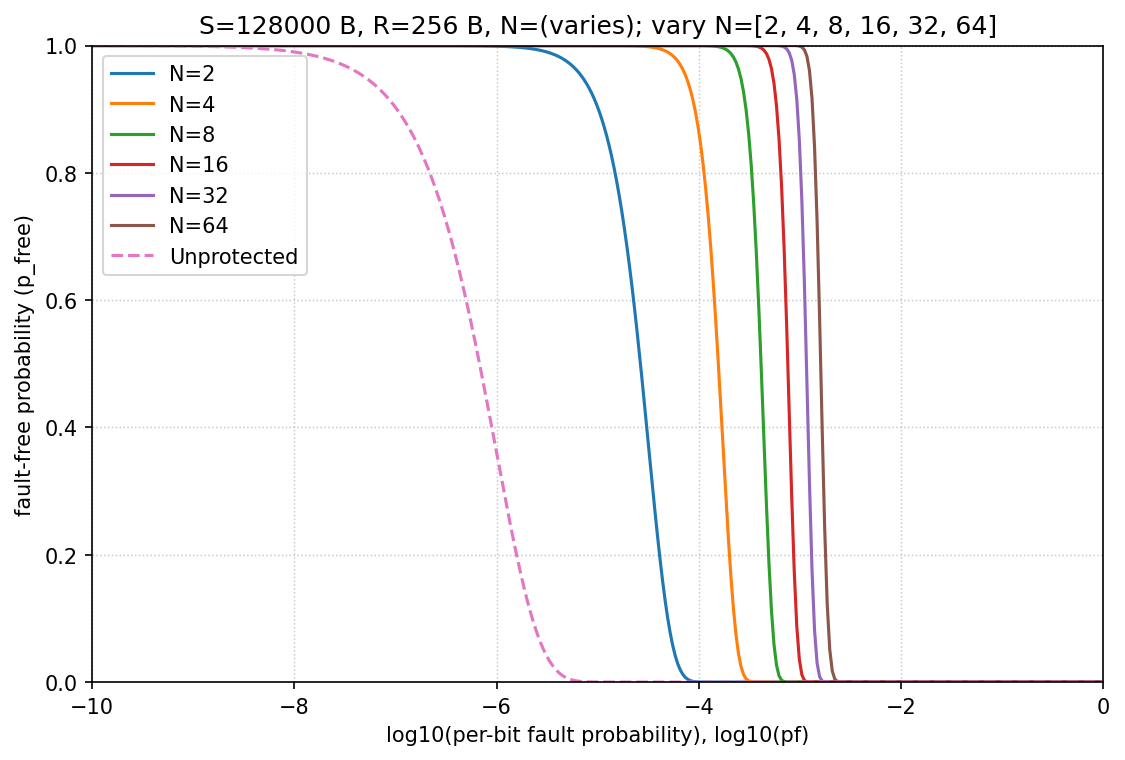
\includegraphics[width=\linewidth]{Chapter-5/figs/pfree_R256_N2_16.png}
  \caption{$p_{\text{free}}$ vs.\ $p_f$ for total memory
           $S=128\,\mathrm{kB}$, fixed region size $R=256$\,B, and
           varying replication count
           $N\in\{2,4,8,16,32,64\}$. Increasing $N$ extends the
           survivability plateau before reliability collapse.}
  \label{fig:varN}
\end{figure}

\begin{figure}[t]
  \centering
  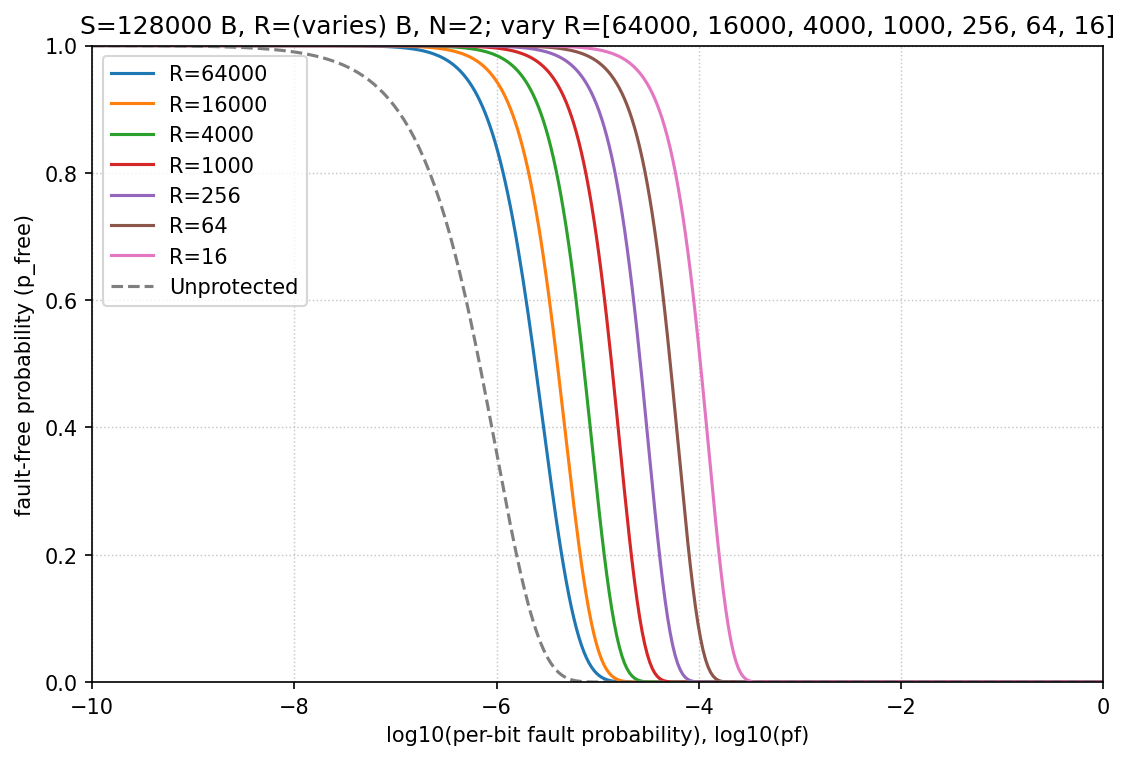
\includegraphics[width=\linewidth]{Chapter-5/figs/pfree_R64k_16_N2.png}
  \caption{$p_{\text{free}}$ vs.\ $p_f$ for total memory
           $S=128\,\mathrm{kB}$, fixed replication count $N=16$,
           and varying region size
           $R\in\{1,2,4,8,16,64\}\,\mathrm{kB}$. Smaller $R$ values
           yield higher survivability due to greater independence.}
  \label{fig:varR}
\end{figure}

These results show that increasing $N$ (replica count) or reducing $R$
(region size) improves the likelihood that at least one intact replica remains.
Smaller regions, however, increase metadata and redirection overhead, defining
a trade-off between granularity and efficiency.

% ---------------------------------------------------
\section{Replication Granularity}
\label{sec:replication-granularity}
% ---------------------------------------------------

Code replication can be organized at multiple \textit{granularities}—each
representing a distinct balance between redundancy cost, validation complexity,
and fault-isolation precision.  Table~\ref{tab:replication-granularity}
summarizes the four principal levels evaluated in this work.

\begin{table}[t]
  \centering
  \small
  \renewcommand{\arraystretch}{1.15}
  \caption{Granularity levels of code replication.}
  \label{tab:replication-granularity}
  \begin{tabularx}{\linewidth}{@{}l P{3.2cm} Y Y@{}}
    \toprule
    \textbf{Granularity} & \textbf{Protected Unit} &
    \textbf{Redirection Mechanism} & \textbf{Typical Use} \\
    \midrule
    Region-Level (RLCR) &
    Entire program image or code partition &
    Startup validation and region selection before execution begins &
    Bootloaders, firmware fallback partitions, redundant ROM images \\

    Function-Level (FLCR) &
    Individual functions &
    Call-site indirection through a validated function table (\texttt{ITab}) &
    Modular executables, dynamic linking, selective runtime recovery \\

    Basic-Block-Level (BBLCR) &
    Control-flow basic blocks &
    Runtime branch redirection through validated block targets (\texttt{BTab}) &
    Fine-grained fault isolation, localized instruction-path recovery \\

    Instruction-Level (ILCR) &
    Individual instructions or micro-sequences &
    On-the-fly reconstruction of instruction bytes followed by immediate
    invocation through generated trampolines or stubs &
    Extreme fault localization; recovery when higher structures are corrupted \\
    \bottomrule
  \end{tabularx}
\end{table}

The hierarchy proceeds from coarse static redundancy (RLCR) to highly dynamic,
self-modifying recovery (ILCR). Each level builds on the previous one by tightening
the granularity of validation and redirection.

% ---------------- RLCR ----------------
\subsection*{Region-Level Code Replication (RLCR)}
At the coarsest level, an entire program image or code region is replicated.
A startup validation routine verifies each region’s integrity and selects the
first valid image for execution. Once a valid region is chosen, execution
proceeds directly within it—no further control-flow indirection is required.
RLCR trades memory capacity for simplicity and is widely used in dual-image
bootloaders and redundant firmware updates.

% ---------------- FLCR ----------------
\subsection*{Function-Level Code Replication (FLCR)}
FLCR divides the program into independently replicated functions.
Indirection occurs only at function-call boundaries, where each call
resolves to a validated function replica before transferring control.
Within a function, execution proceeds directly with no additional
redirection.

% ---------------- BBLCR ----------------
\subsection*{Basic-Block-Level Code Replication (BBLCR)}
BBLCR refines FLCR by introducing indirection at basic-block boundaries.
Each branch or jump target is resolved at runtime to a verified replica,
while instructions within a basic block execute directly.
This fine-grained indirection enables execution to bypass damaged code
regions within a function and continue safely through valid paths.

% ---------------- ILCR ----------------
% ---------------- ILCR ----------------
\subsection*{Instruction-Level Code Replication (ILCR)}
At the finest granularity, ILCR reconstructs instructions dynamically rather
than redirecting among existing blocks. Short instruction sequences are
regenerated from redundant encodings or reference data, placed into writable
memory, validated, and immediately invoked via a temporary trampoline.
Because execution enters synthesized code directly, ILCR behaves like a
disciplined form of self-modifying code.

This capability requires several architectural conditions:

\begin{itemize}
  \item \textbf{Writable or relocatable code space:}
        Reconstructed instructions must reside in a writable and executable
        memory region, or the system must relocate code dynamically into such
        a space at runtime.

  \item \textbf{No PC-relative addressing:}
        Reconstructed sequences must avoid PC-relative addressing or be fully
        position-independent, since relocation invalidates absolute offsets.
        All references must be expressed through registers or absolute pointers.

  \item \textbf{Controlled reconstruction:}
        Each reconstructed fragment is verified for integrity before execution
        and discarded or replaced after completion, preventing uncontrolled
        self-modification.
\end{itemize}

At this granularity, ILCR resembles a form of \textbf{code repair} rather than
traditional replication. Because its mechanisms focus on dynamic regeneration
and repair rather than redirection among preexisting copies, ILCR lies beyond
the scope of the replication-focused analysis in this study.

% ---------------------------------------------------
\section{Summary}
\label{sec:replication-summary}
% ---------------------------------------------------

This chapter established the analytical foundation of code replication and its
hierarchical structure. The probabilistic model quantified how redundancy
parameters ($R$, $N$) determine survivability, while the granularity taxonomy
(RLCR, FLCR, BBLCR) illustrates how runtime control-flow management evolves—
from region-level selection through function-call redirection to basic-block-level
edge resolution.

Across all three levels, the total amount of redundant code storage remains
constant; what differs is the point in the control flow where redirection
occurs. RLCR performs selection at the region boundary, FLCR redirects at
function-call sites, and BBLCR introduces indirection at basic-block edges.
This progression refines how faults are isolated and bypassed without increasing
replication overhead.

The following chapters examine each level in detail:
\begin{itemize}
  \item Chapter~\ref{chap:region-level} — \textbf{Region-Level Replication (RLCR)}
        enabling recovery through region-level selection at runtime.
  \item Chapter~\ref{chap:flcr} — \textbf{Function-Level Replication (FLCR)}
        introducing call-site redirection to isolate faults within specific
        functions.
  \item Chapter~\ref{chap:bblcr} — \textbf{Basic-Block-Level Replication (BBLCR)}
        extending redirection to intra-function control flow for fine-grained
        fault recovery.
\end{itemize}

Together, these mechanisms form a continuum of software-based fault-tolerance
strategies, in which finer granularities provide greater control-flow resilience
without additional redundancy cost, but at the expense of increased runtime
and management complexity.